% Options for packages loaded elsewhere
\PassOptionsToPackage{unicode}{hyperref}
\PassOptionsToPackage{hyphens}{url}
\PassOptionsToPackage{dvipsnames,svgnames,x11names}{xcolor}
%
\documentclass[
]{article}
\usepackage{amsmath,amssymb}
\usepackage{fancyvrb}
\usepackage{fvextra}
%\RecustomVerbatimEnvironment{verbatim}{Verbatim}{commandchars=\\\{\}}
\usepackage{lmodern}
\usepackage{bold-extra}
\usepackage{iftex}
\ifPDFTeX
  \usepackage[T1]{fontenc}
  \usepackage[utf8]{inputenc}
  \usepackage{textcomp} % provide euro and other symbols
\else % if luatex or xetex
  \usepackage{unicode-math}
  \defaultfontfeatures{Scale=MatchLowercase}
  \defaultfontfeatures[\rmfamily]{Ligatures=TeX,Scale=1}
\fi
% Use upquote if available, for straight quotes in verbatim environments
\IfFileExists{upquote.sty}{\usepackage{upquote}}{}
\IfFileExists{microtype.sty}{% use microtype if available
  \usepackage[]{microtype}
  \UseMicrotypeSet[protrusion]{basicmath} % disable protrusion for tt fonts
}{}
\makeatletter
\@ifundefined{KOMAClassName}{% if non-KOMA class
  \IfFileExists{parskip.sty}{%
    \usepackage{parskip}
  }{% else
    \setlength{\parindent}{0pt}
    \setlength{\parskip}{6pt plus 2pt minus 1pt}}
}{% if KOMA class
  \KOMAoptions{parskip=half}}
\makeatother
\usepackage{xcolor}
\usepackage{graphicx}
\makeatletter
\def\maxwidth{\ifdim\Gin@nat@width>\linewidth\linewidth\else\Gin@nat@width\fi}
\def\maxheight{\ifdim\Gin@nat@height>\textheight\textheight\else\Gin@nat@height\fi}
\makeatother
% Scale images if necessary, so that they will not overflow the page
% margins by default, and it is still possible to overwrite the defaults
% using explicit options in \includegraphics[width, height, ...]{}
\setkeys{Gin}{width=\maxwidth,height=\maxheight,keepaspectratio}
% Set default figure placement to htbp
\makeatletter
\def\fps@figure{htbp}
\makeatother
\setlength{\emergencystretch}{3em} % prevent overfull lines
\providecommand{\tightlist}{%
  \setlength{\itemsep}{0pt}\setlength{\parskip}{0pt}}
\setcounter{secnumdepth}{5}
\makeatletter
\@ifpackageloaded{subfig}{}{\usepackage{subfig}}
\@ifpackageloaded{caption}{}{\usepackage{caption}}
\captionsetup[subfloat]{margin=0.5em}
\AtBeginDocument{%
\renewcommand*\figurename{Figure}
\renewcommand*\tablename{Table}
}
\AtBeginDocument{%
\renewcommand*\listfigurename{List of Figures}
\renewcommand*\listtablename{List of Tables}
}
\newcounter{pandoccrossref@subfigures@footnote@counter}
\newenvironment{pandoccrossrefsubfigures}{%
\setcounter{pandoccrossref@subfigures@footnote@counter}{0}
\begin{figure}\centering%
\gdef\global@pandoccrossref@subfigures@footnotes{}%
\DeclareRobustCommand{\footnote}[1]{\footnotemark%
\stepcounter{pandoccrossref@subfigures@footnote@counter}%
\ifx\global@pandoccrossref@subfigures@footnotes\empty%
\gdef\global@pandoccrossref@subfigures@footnotes{{##1}}%
\else%
\g@addto@macro\global@pandoccrossref@subfigures@footnotes{, {##1}}%
\fi}}%
{\end{figure}%
\addtocounter{footnote}{-\value{pandoccrossref@subfigures@footnote@counter}}
\@for\f:=\global@pandoccrossref@subfigures@footnotes\do{\stepcounter{footnote}\footnotetext{\f}}%
\gdef\global@pandoccrossref@subfigures@footnotes{}}
\@ifpackageloaded{float}{}{\usepackage{float}}
\floatstyle{ruled}
\@ifundefined{c@chapter}{\newfloat{codelisting}{h}{lop}}{\newfloat{codelisting}{h}{lop}[chapter]}
\floatname{codelisting}{Listing}
\newcommand*\listoflistings{\listof{codelisting}{List of Listings}}
\makeatother
\ifLuaTeX
  \usepackage{selnolig}  % disable illegal ligatures
\fi
\IfFileExists{bookmark.sty}{\usepackage{bookmark}}{\usepackage{hyperref}}
\IfFileExists{xurl.sty}{\usepackage{xurl}}{} % add URL line breaks if available
\urlstyle{same} % disable monospaced font for URLs
\hypersetup{
  pdftitle={A Simple 3D Puzzle},
  pdfauthor={Tyler Neylon},
  colorlinks=true,
  linkcolor={black},
  filecolor={Maroon},
  citecolor={Blue},
  urlcolor={Blue},
  pdfcreator={LaTeX via pandoc}}

\title{A Simple 3D Puzzle}
\author{Tyler Neylon}
\date{\href{https://tylerneylon.com/a/7date/}{345.2023}}

%%%%%%%%%%%%%%%%%%%%%%%%%%%%%%%%%%%%%%%%%%%%%%%%%%%%%%%%%%%%%%%%%%%%%%%%%%%
% Begin custom, non-pandoc commands.

\newcommand{\customstrut}{\rule[-3mm]{0mm}{7.5mm}}
\newenvironment{densearray}{\begin{array}{rcl}}{\end{array}}
\newcommand{\class}[1]{}
\newcommand{\Rule}[3]{}
\newcommand{\optquad}{\quad}
\newcommand{\smallscrneg}{}
\newcommand{\smallscr}[1]{}
\newcommand{\bigscr}[1]{#1}
\newcommand{\smallscrskip}[1]{}

% I learned some things from these two links:
% https://tex.stackexchange.com/questions/145812/using-fbox-in-a-newenvironment
% https://tex.stackexchange.com/questions/120042/splitting-a-command-syntax-across-a-newenvironment-definition

\newsavebox{\mybox}
\newenvironment{myboxed}{\begin{lrbox}{\mybox}\begin{minipage}{0.98\textwidth}}{\end{minipage}\end{lrbox}\fbox{\usebox{\mybox}}}

\newcommand{\boxedstart}{\begin{myboxed}}
\newcommand{\boxedend}{\end{myboxed}}

\newcommand{\crossedouty}{\dot y \kern -4.5pt \raise 4.9pt \hbox{\(\scriptscriptstyle\diagup\)}}
\newcommand{\crossedoutone}{\dot 1 \kern -5.1pt \raise 6.6pt \hbox{\(\scriptscriptstyle\diagup\)}}
\newcommand{\crossedouttwo}{\dot 2 \kern -5.1pt \raise 6.6pt \hbox{\(\scriptscriptstyle\diagup\)}}
\newcommand{\crossedoutthree}{\dot 3 \kern -5.1pt \raise 6.6pt \hbox{\(\scriptscriptstyle\diagup\)}}
\newcommand{\crossedoutfive}{\dot 5 \kern -5.1pt \raise 6.6pt \hbox{\(\scriptscriptstyle\diagup\)}}
\newcommand{\crossedoutsix}{\dot 6 \kern -5.1pt \raise 6.6pt \hbox{\(\scriptscriptstyle\diagup\)}}
\newcommand{\crossedoutseven}{\dot 7 \kern -5.1pt \raise 6.6pt \hbox{\(\scriptscriptstyle\diagup\)}}
\newcommand{\lowerhaty}{\lower 1ex\hbox{\(\hat y\)}}
\newcommand{\lhy}{\lower 1ex\hbox{\(\hat y\)}}

\let\smallstart\iffalse
\let\smallend\fi

% End custom, non-pandoc commands.
%%%%%%%%%%%%%%%%%%%%%%%%%%%%%%%%%%%%%%%%%%%%%%%%%%%%%%%%%%%%%%%%%%%%%%%%%%%

\begin{document}
\maketitle

\newcommand{\R}{\mathbb{R}}
\newcommand{\N}{\mathbb{N}}
\newcommand{\eqnset}[1]{\left.\mbox{$#1$}\;\;\right\rbrace\class{postbrace}{ }}
\providecommand{\latexonlyrule}[3][]{}
\providecommand{\optquad}{\class{optquad}{}}
\providecommand{\smallscrneg}{\class{smallscrneg}{ }}
\providecommand{\bigscr}[1]{\class{bigscr}{#1}}
\providecommand{\smallscr}[1]{\class{smallscr}{#1}}
\providecommand{\smallscrskip}[1]{\class{smallscrskip}{\hskip #1}}

\newcommand{\mydots}{{\cdot}\kern -0.1pt{\cdot}\kern -0.1pt{\cdot}}

\newcommand{\?}{\stackrel{?}{=}}
\newcommand{\sign}{\textsf{sign}}
\newcommand{\order}{\textsf{order}}
\newcommand{\flips}{\textsf{flips}}
\newcommand{\samecycles}{\textsf{same$\\\_$cycles}}
\newcommand{\canon}{\textsf{canon}}
\newcommand{\cs}{\mathsf{cs}}
\newcommand{\dist}{\mathsf{dist}}
\renewcommand{\theenumi}{(\roman{enumi})}

{[} Formats:
\href{http://tylerneylon.com/a/lego_puzzle/lego_puzzle.html}{html}
\textbar{}
\href{http://tylerneylon.com/a/lego_puzzle/lego_puzzle.pdf}{pdf}
\(\,\){]}

\hypertarget{the-puzzle}{%
\section{The Puzzle}\label{the-puzzle}}

Here's a fun puzzle: Take six boxes, each \(1\times 2\times 2\) in size,
and find a way to pack them into a \(3\times 3\times 3\) cube.

\begin{center}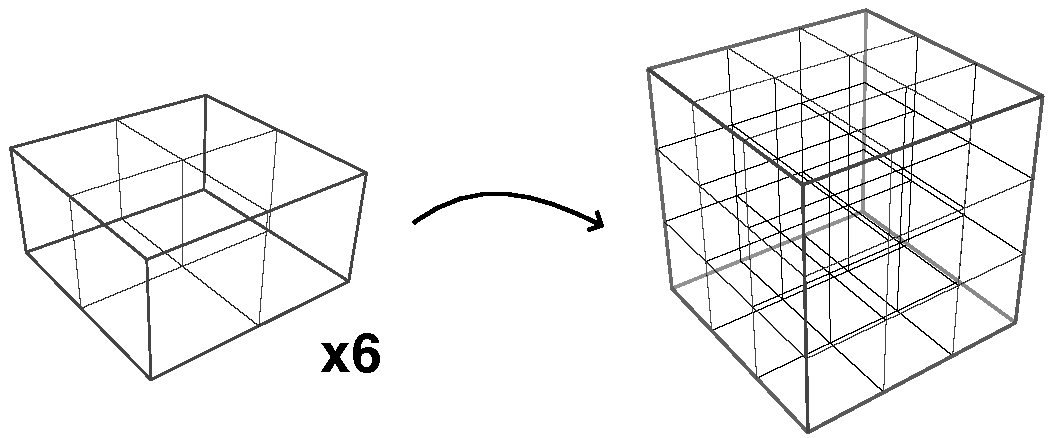
\includegraphics[width=0.5\textwidth]{img/img1.pdf}\end{center}

I learned about this puzzle through Donald Knuth's \emph{The Art of
Computer Programming,} \(\S 7.2.2.1\). The six boxes have a total volume
of 24 cubies (I'll call a \(1\times 1\times 1\) unit a ``cubie,'' as
Knuth does). They certainly have a chance of fitting into the 27 cubie
spaces of the larger \(3\times 3\times 3\) volume. But the initial
configurations I tried failed to fit more than five boxes in the space
allowed:

\begin{center}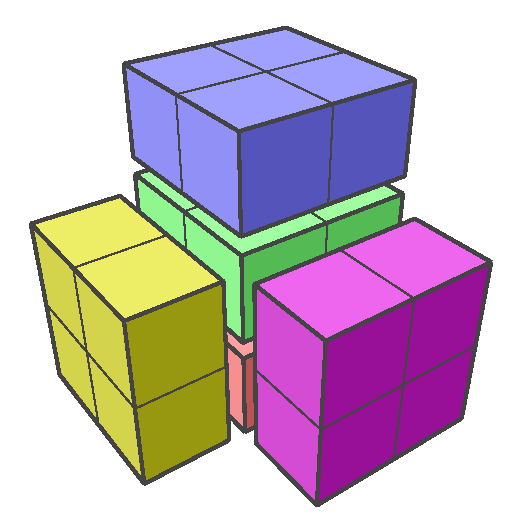
\includegraphics[width=0.5\textwidth]{img/img2.pdf}\end{center}

You might be able to solve this by simply thinking about it. But it's
even more fun to play with a physical model. \newline Did you know that
a \(2\times 2\) Lego brick with 2 tile-heights on top forms a perfect
cube?

\begin{center}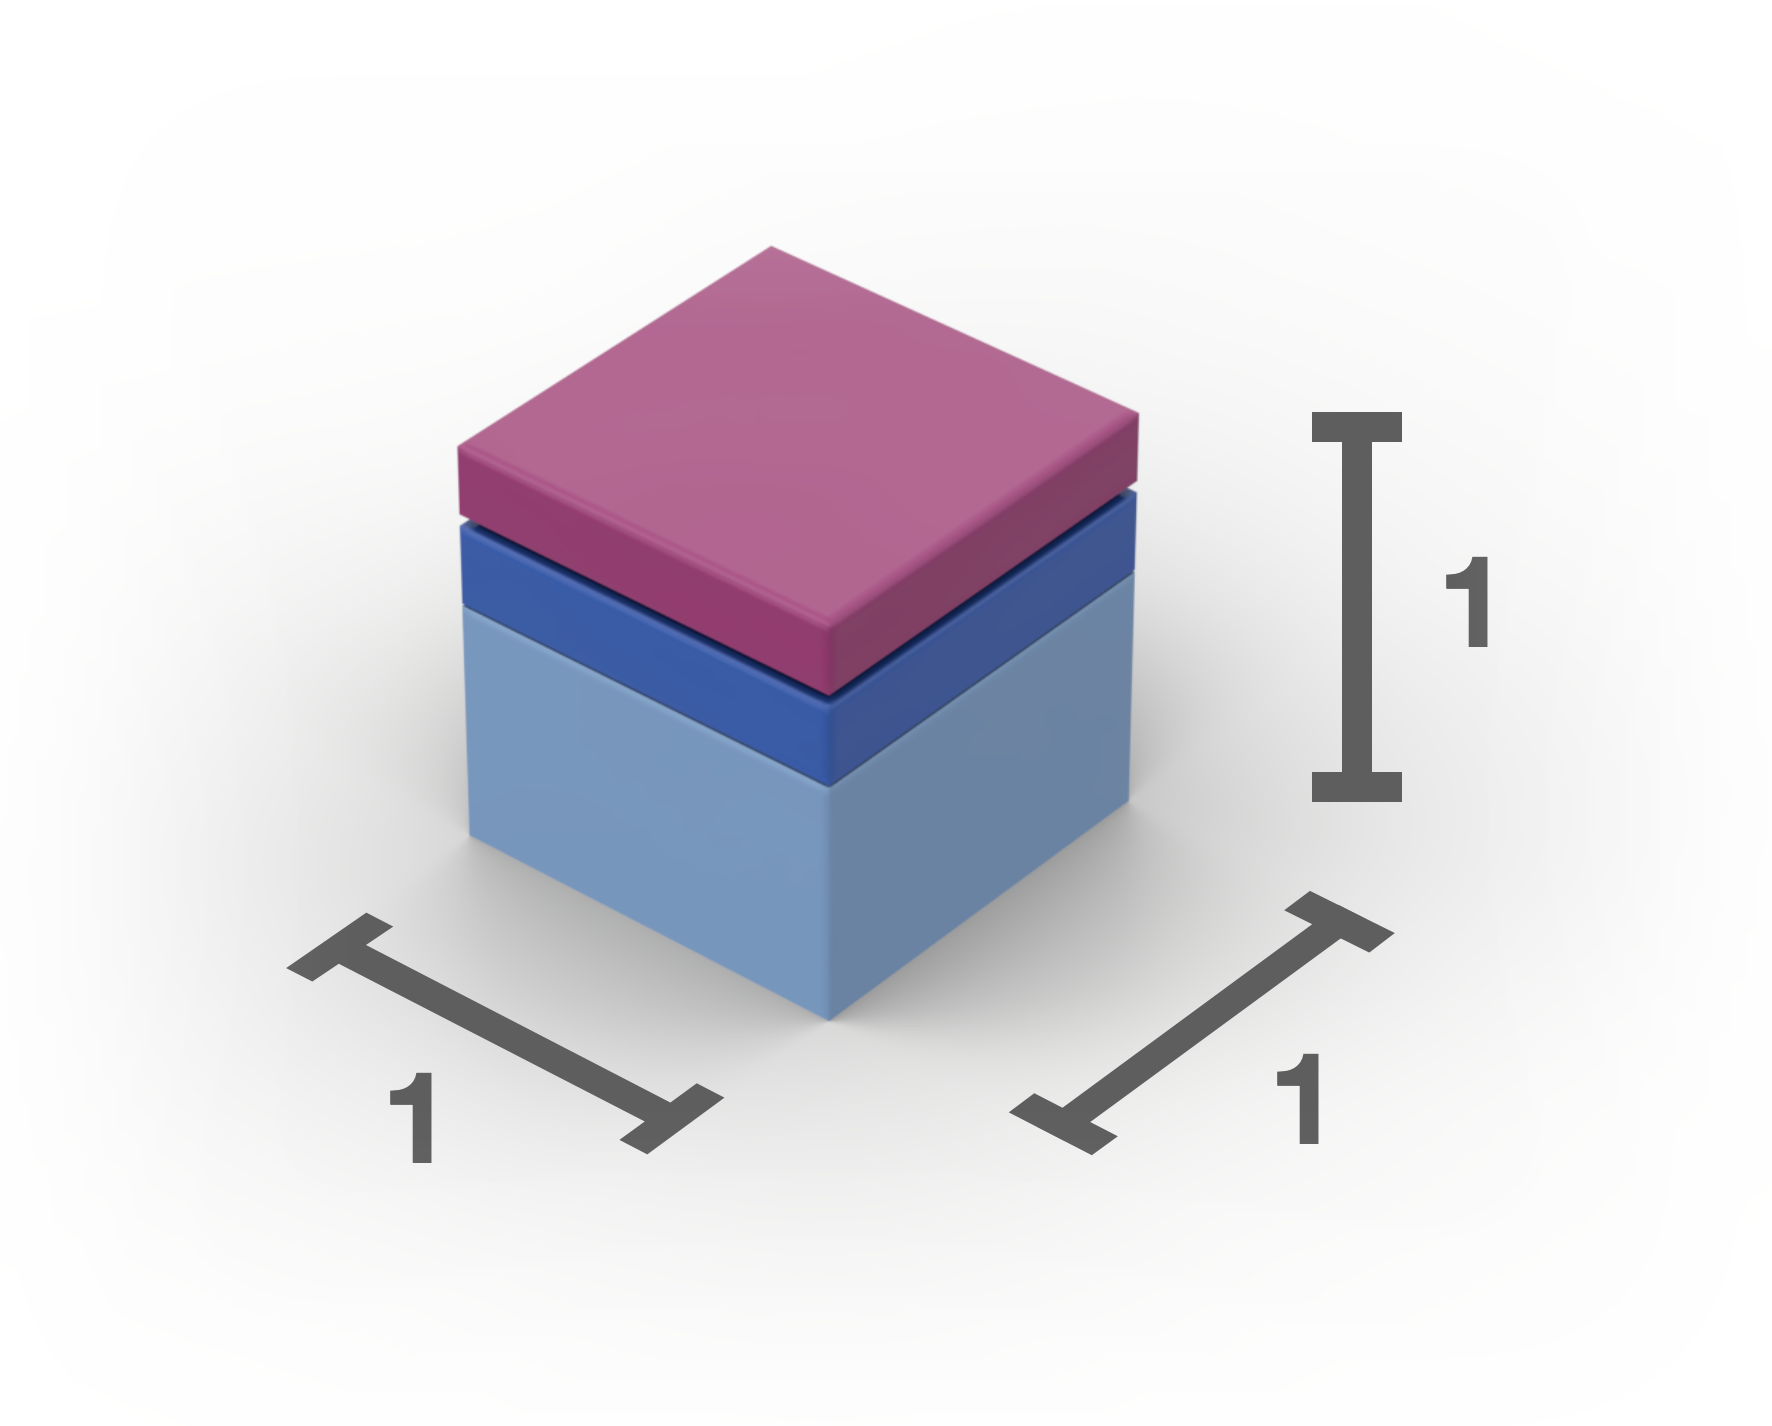
\includegraphics[width=0.5\textwidth]{img/annotated_lego_cube.png}\end{center}

This allows us to construct the puzzle like so:

\begin{center}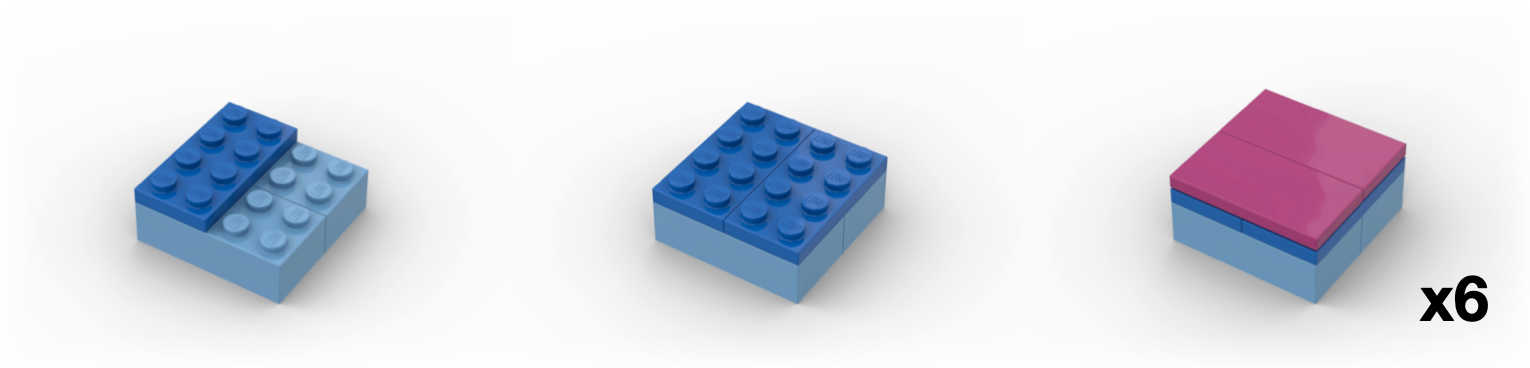
\includegraphics[width=0.9\textwidth,height=\textheight]{img/piece_steps2.png}\end{center}
\begin{center}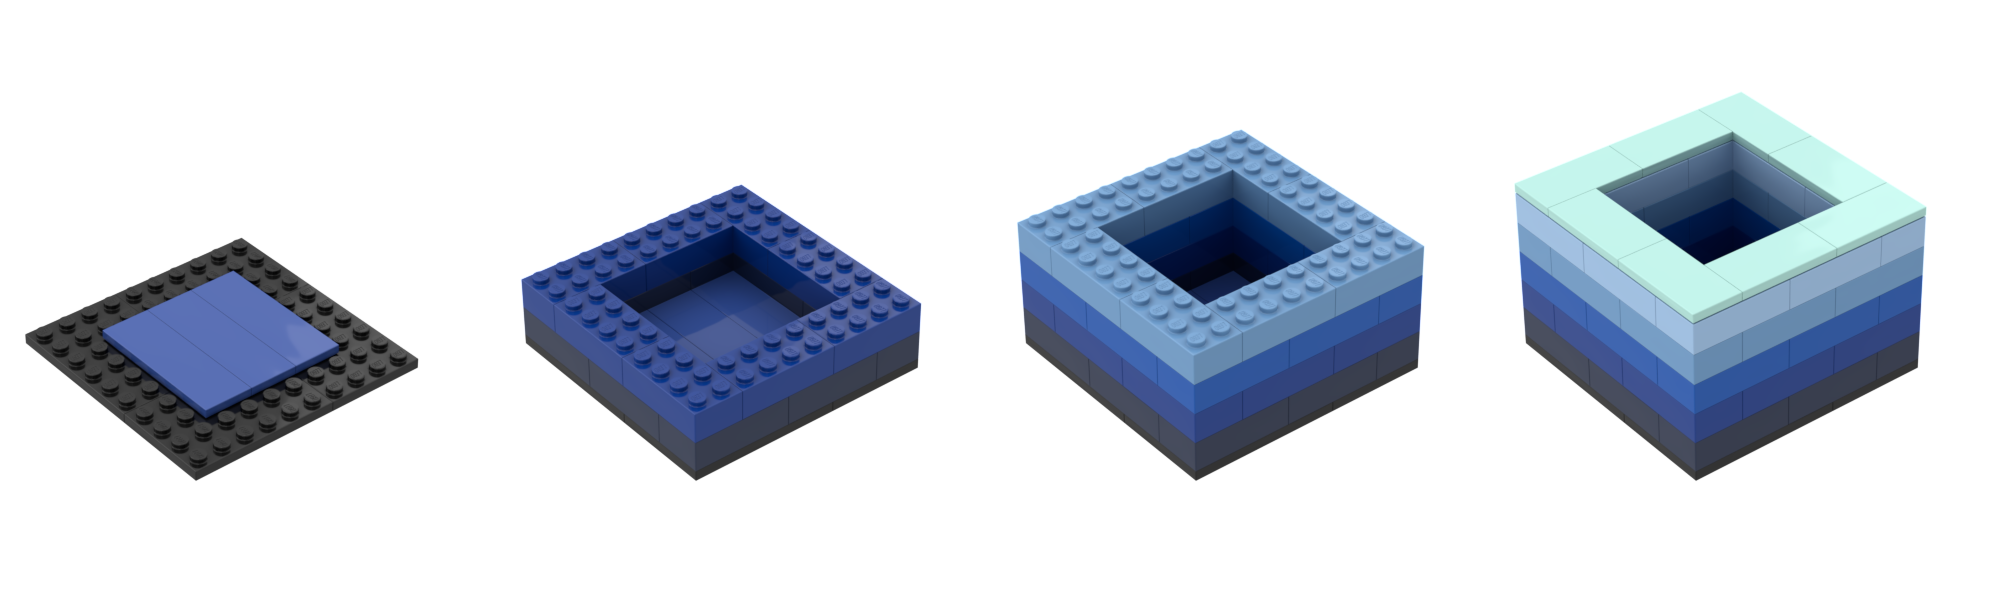
\includegraphics[width=0.9\textwidth,height=\textheight]{img/puzzle_box_steps.png}\end{center}

Here's the hodgepodge model I built with my kids' Legos:

\begin{center}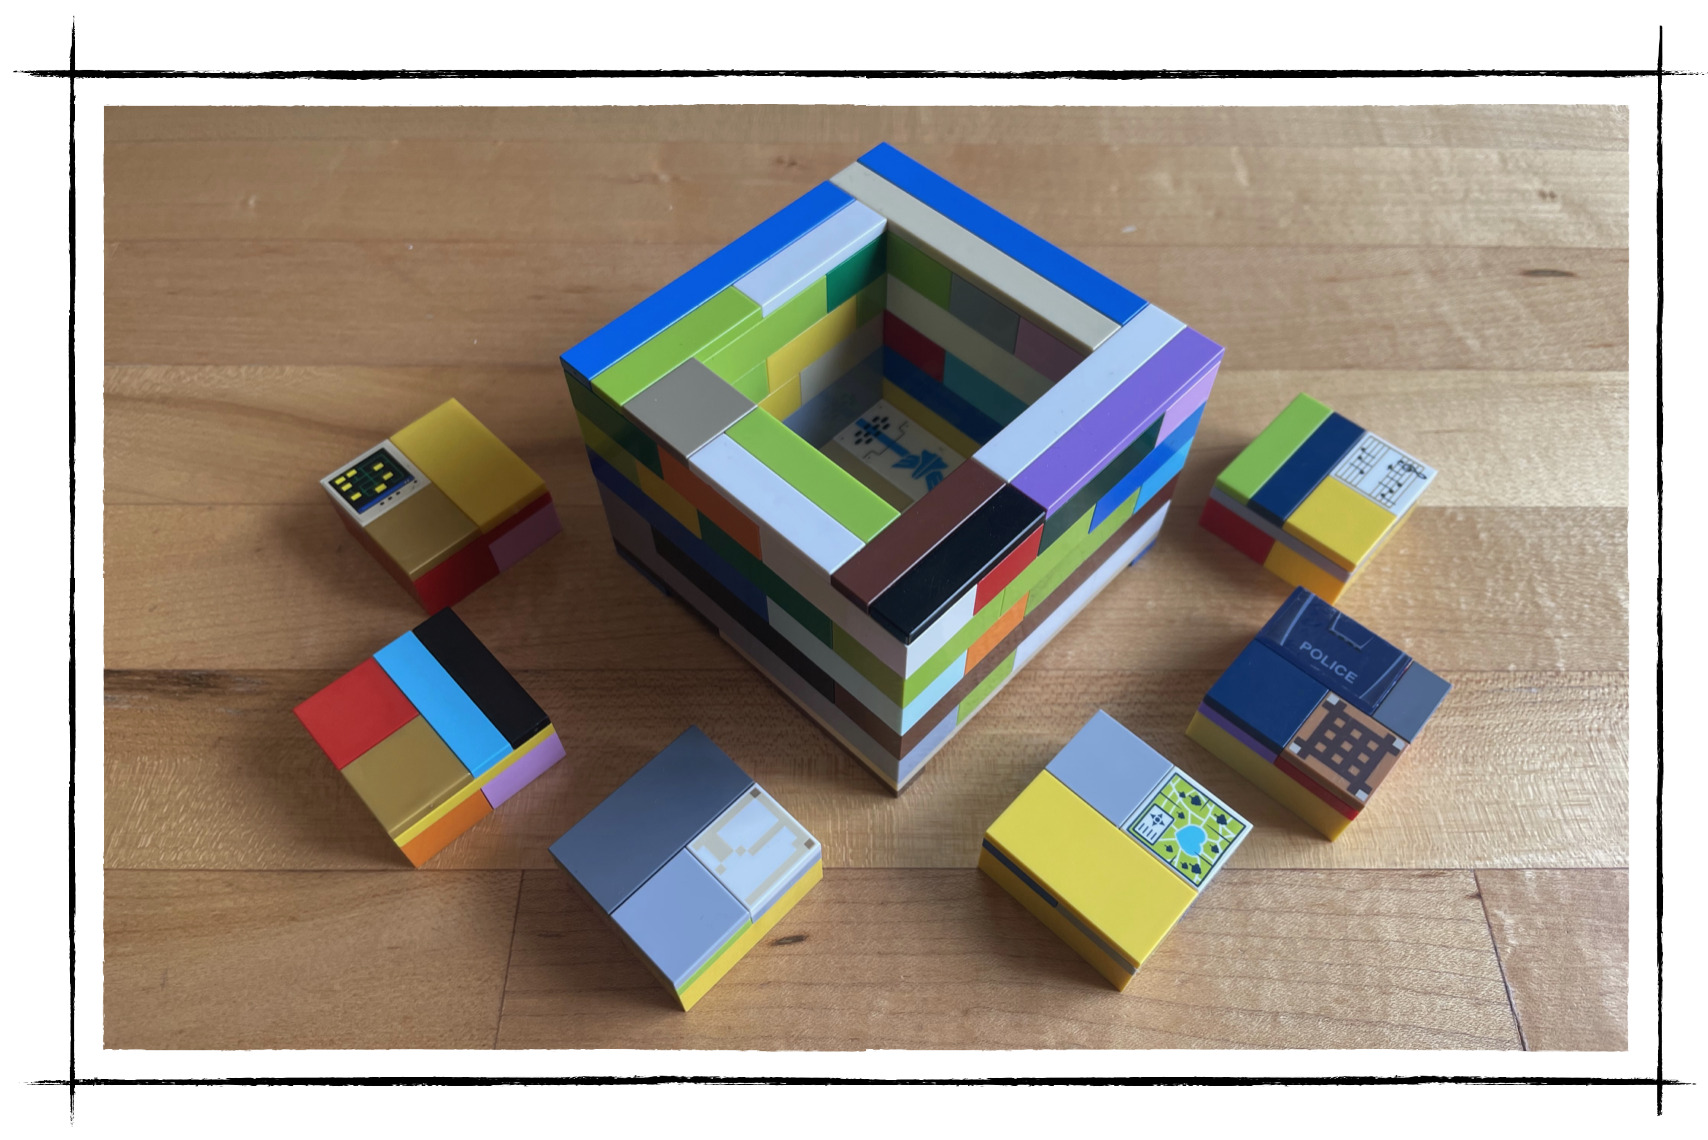
\includegraphics[width=0.7\textwidth]{img/home_model.jpg}\end{center}

I'll write a little about the math behind this puzzle below, but for now
I'll give you a vertical break so you don't accidentally see the
solution. Try out the puzzle first!

~ \vspace{1in}

\begin{center}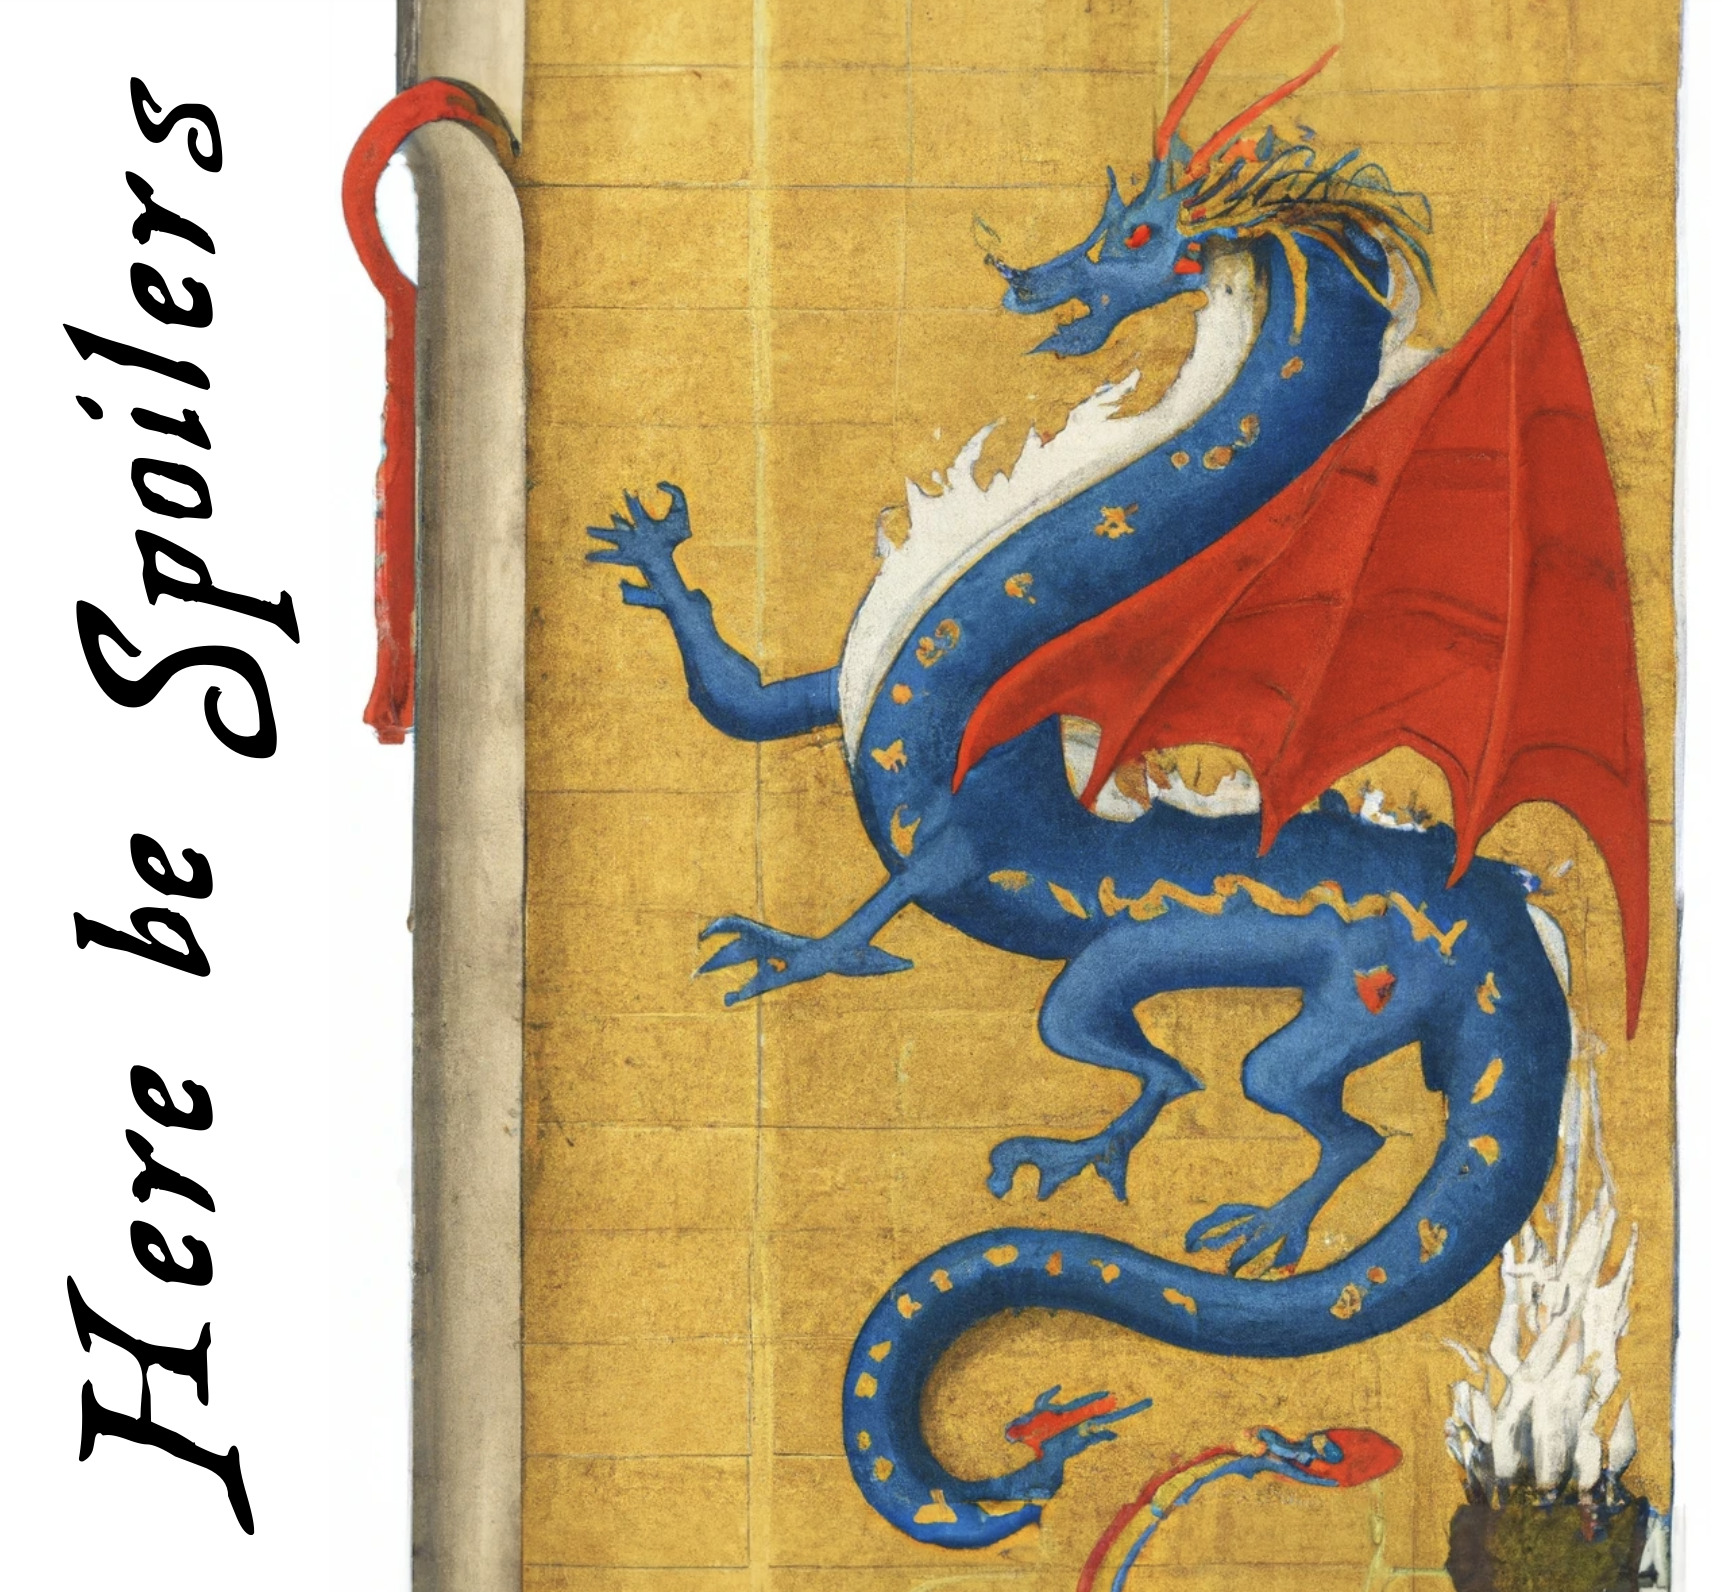
\includegraphics[width=0.9\textwidth,height=\textheight]{img/here_be_spoilers.jpg}\end{center}

~ \newpage

\hypertarget{the-solution}{%
\section{The Solution}\label{the-solution}}

Next part of the article.

\end{document}

